\documentclass{standalone}
\usepackage{tikz}
\usetikzlibrary{patterns, positioning}


\begin{document}
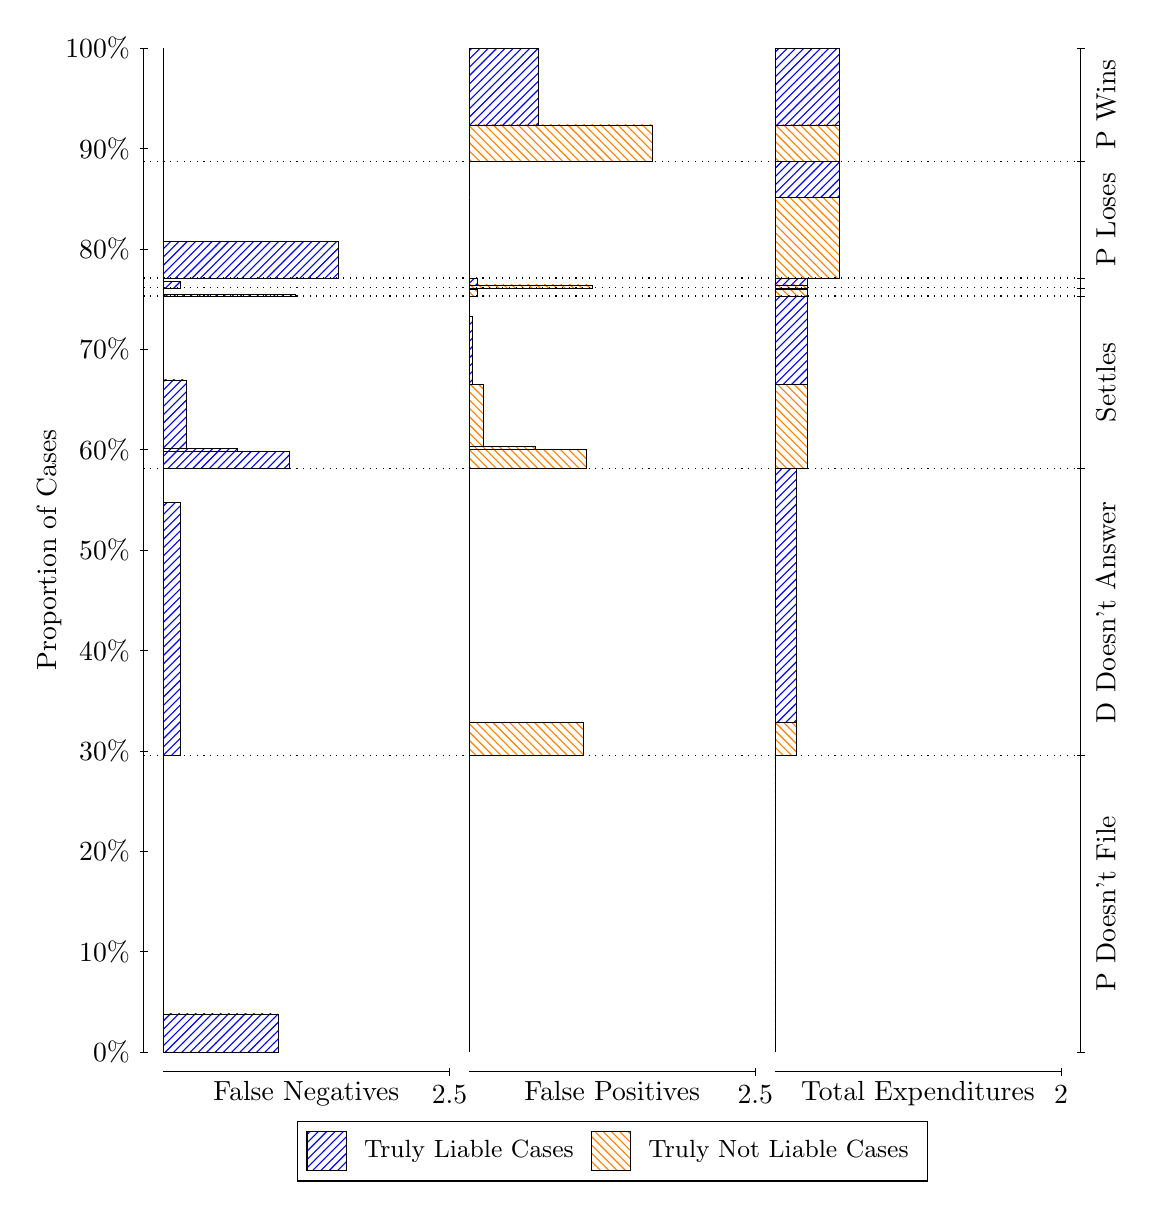
\begin{tikzpicture}
\draw[black, very thin] (1.5,1.75) -- (1.5,14.5);
\node[rotate=90, text=black, anchor=center] at (0.3, 8.125) {Proportion of Cases};
\draw[black, very thin] (1.45,1.75) -- (1.55,1.75);
\node[text=black, anchor=east] at (1.45, 1.75) {0\%};
\draw[black, very thin] (1.45,3.025) -- (1.55,3.025);
\node[text=black, anchor=east] at (1.45, 3.025) {10\%};
\draw[black, very thin] (1.45,4.3) -- (1.55,4.3);
\node[text=black, anchor=east] at (1.45, 4.3) {20\%};
\draw[black, very thin] (1.45,5.575) -- (1.55,5.575);
\node[text=black, anchor=east] at (1.45, 5.575) {30\%};
\draw[black, very thin] (1.45,6.85) -- (1.55,6.85);
\node[text=black, anchor=east] at (1.45, 6.85) {40\%};
\draw[black, very thin] (1.45,8.125) -- (1.55,8.125);
\node[text=black, anchor=east] at (1.45, 8.125) {50\%};
\draw[black, very thin] (1.45,9.4) -- (1.55,9.4);
\node[text=black, anchor=east] at (1.45, 9.4) {60\%};
\draw[black, very thin] (1.45,10.675) -- (1.55,10.675);
\node[text=black, anchor=east] at (1.45, 10.675) {70\%};
\draw[black, very thin] (1.45,11.95) -- (1.55,11.95);
\node[text=black, anchor=east] at (1.45, 11.95) {80\%};
\draw[black, very thin] (1.45,13.225) -- (1.55,13.225);
\node[text=black, anchor=east] at (1.45, 13.225) {90\%};
\draw[black, very thin] (1.45,14.5) -- (1.55,14.5);
\node[text=black, anchor=east] at (1.45, 14.5) {100\%};

\draw[black, very thin] (13.4,1.75) -- (13.4,14.5);
\draw[black, very thin] (13.35,1.75) -- (13.45,1.75);
\node[anchor=west] at (13.35, 1.75) {};
\draw[black, very thin] (13.35,5.5119) -- (13.45,5.5119);
\node[anchor=west] at (13.35, 5.5119) {};
\draw[black, very thin] (13.35,9.1605) -- (13.45,9.1605);
\node[anchor=west] at (13.35, 9.1605) {};
\draw[black, very thin] (13.35,11.351) -- (13.45,11.351);
\node[anchor=west] at (13.35, 11.351) {};
\draw[black, very thin] (13.35,11.455) -- (13.45,11.455);
\node[anchor=west] at (13.35, 11.455) {};
\draw[black, very thin] (13.35,11.579) -- (13.45,11.579);
\node[anchor=west] at (13.35, 11.579) {};
\draw[black, very thin] (13.35,13.063) -- (13.45,13.063);
\node[anchor=west] at (13.35, 13.063) {};
\draw[black, very thin] (13.35,14.5) -- (13.45,14.5);
\node[anchor=west] at (13.35, 14.5) {};

\draw[black, very thin, pattern color=blue, pattern=north east lines] (1.75,1.75) rectangle (3.2033,2.2345);
\draw[black, very thin, pattern color=orange, pattern=north west lines] (1.75,2.2345) rectangle (1.75,5.5119);
\draw[black, very thin, pattern color=blue, pattern=north east lines] (1.75,5.5119) rectangle (1.968,8.7326);
\draw[black, very thin, pattern color=orange, pattern=north west lines] (1.75,8.7326) rectangle (1.75,9.1605);
\draw[black, very thin, pattern color=blue, pattern=north east lines] (1.75,9.1605) rectangle (3.3487,9.3729);
\draw[black, very thin, pattern color=blue, pattern=north east lines] (1.75,9.3729) rectangle (2.6947,9.4185);
\draw[black, very thin, pattern color=blue, pattern=north east lines] (1.75,9.4185) rectangle (2.0407,10.286);
\draw[black, very thin, pattern color=orange, pattern=north west lines] (1.75,10.286) rectangle (1.75,11.351);
\draw[black, very thin, pattern color=blue, pattern=north east lines] (1.75,11.351) rectangle (3.4213,11.373);
\draw[black, very thin, pattern color=orange, pattern=north west lines] (1.75,11.373) rectangle (1.75,11.455);
\draw[black, very thin, pattern color=blue, pattern=north east lines] (1.75,11.455) rectangle (1.968,11.54);
\draw[black, very thin, pattern color=orange, pattern=north west lines] (1.75,11.54) rectangle (1.75,11.579);
\draw[black, very thin, pattern color=blue, pattern=north east lines] (1.75,11.579) rectangle (3.9663,12.04);
\draw[black, very thin, pattern color=orange, pattern=north west lines] (1.75,12.04) rectangle (1.75,13.063);
\draw[black, very thin, pattern color=orange, pattern=north west lines] (1.75,13.063) rectangle (1.75,13.524);
\draw[black, very thin, pattern color=blue, pattern=north east lines] (1.75,13.524) rectangle (1.75,14.5);
\draw[black, very thin, pattern color=orange, pattern=north west lines] (5.6333,1.75) rectangle (5.6333,5.0274);
\draw[black, very thin, pattern color=blue, pattern=north east lines] (5.6333,5.0274) rectangle (5.6333,5.5119);
\draw[black, very thin, pattern color=orange, pattern=north west lines] (5.6333,5.5119) rectangle (7.0867,5.9398);
\draw[black, very thin, pattern color=blue, pattern=north east lines] (5.6333,5.9398) rectangle (5.6333,9.1605);
\draw[black, very thin, pattern color=orange, pattern=north west lines] (5.6333,9.1605) rectangle (7.123,9.4);
\draw[black, very thin, pattern color=orange, pattern=north west lines] (5.6333,9.4) rectangle (6.469,9.4456);
\draw[black, very thin, pattern color=orange, pattern=north west lines] (5.6333,9.4456) rectangle (5.815,10.226);
\draw[black, very thin, pattern color=blue, pattern=north east lines] (5.6333,10.226) rectangle (5.6697,11.093);
\draw[black, very thin, pattern color=blue, pattern=north east lines] (5.6333,11.093) rectangle (5.6333,11.351);
\draw[black, very thin, pattern color=orange, pattern=north west lines] (5.6333,11.351) rectangle (5.7423,11.433);
\draw[black, very thin, pattern color=blue, pattern=north east lines] (5.6333,11.433) rectangle (5.6333,11.455);
\draw[black, very thin, pattern color=orange, pattern=north west lines] (5.6333,11.455) rectangle (7.1957,11.493);
\draw[black, very thin, pattern color=blue, pattern=north east lines] (5.6333,11.493) rectangle (5.7423,11.579);
\draw[black, very thin, pattern color=orange, pattern=north west lines] (5.6333,11.579) rectangle (5.6333,12.602);
\draw[black, very thin, pattern color=blue, pattern=north east lines] (5.6333,12.602) rectangle (5.6333,13.063);
\draw[black, very thin, pattern color=orange, pattern=north west lines] (5.6333,13.063) rectangle (7.9587,13.524);
\draw[black, very thin, pattern color=blue, pattern=north east lines] (5.6333,13.524) rectangle (6.5053,14.5);
\draw[black, very thin, pattern color=orange, pattern=north west lines] (9.5167,1.75) rectangle (9.5167,5.0274);
\draw[black, very thin, pattern color=blue, pattern=north east lines] (9.5167,5.0274) rectangle (9.5167,5.5119);
\draw[black, very thin, pattern color=orange, pattern=north west lines] (9.5167,5.5119) rectangle (9.7892,5.9398);
\draw[black, very thin, pattern color=blue, pattern=north east lines] (9.5167,5.9398) rectangle (9.7892,9.1605);
\draw[black, very thin, pattern color=orange, pattern=north west lines] (9.5167,9.1605) rectangle (9.9254,10.226);
\draw[black, very thin, pattern color=blue, pattern=north east lines] (9.5167,10.226) rectangle (9.9254,11.351);
\draw[black, very thin, pattern color=orange, pattern=north west lines] (9.5167,11.351) rectangle (9.9254,11.433);
\draw[black, very thin, pattern color=blue, pattern=north east lines] (9.5167,11.433) rectangle (9.9254,11.455);
\draw[black, very thin, pattern color=orange, pattern=north west lines] (9.5167,11.455) rectangle (9.9254,11.493);
\draw[black, very thin, pattern color=blue, pattern=north east lines] (9.5167,11.493) rectangle (9.9254,11.579);
\draw[black, very thin, pattern color=orange, pattern=north west lines] (9.5167,11.579) rectangle (10.334,12.602);
\draw[black, very thin, pattern color=blue, pattern=north east lines] (9.5167,12.602) rectangle (10.334,13.063);
\draw[black, very thin, pattern color=orange, pattern=north west lines] (9.5167,13.063) rectangle (10.334,13.524);
\draw[black, very thin, pattern color=blue, pattern=north east lines] (9.5167,13.524) rectangle (10.334,14.5);
\draw[black, dotted] (1.5,5.5119) -- (13.4,5.5119);
\draw[black, dotted] (1.5,9.1605) -- (13.4,9.1605);
\draw[black, dotted] (1.5,11.351) -- (13.4,11.351);
\draw[black, dotted] (1.5,11.455) -- (13.4,11.455);
\draw[black, dotted] (1.5,11.579) -- (13.4,11.579);
\draw[black, dotted] (1.5,13.063) -- (13.4,13.063);
\draw[black, very thin] (1.75,1.5) -- (5.3833,1.5);
\node[text=black, anchor=north] at (3.5667, 1.5) {False Negatives};
\draw[black, very thin] (5.3833,1.45) -- (5.3833,1.55);
\node[text=black, anchor=north] at (5.3833, 1.45) {2.5};

\draw[black, very thin] (5.6333,1.5) -- (9.2667,1.5);
\node[text=black, anchor=north] at (7.45, 1.5) {False Positives};
\draw[black, very thin] (9.2667,1.45) -- (9.2667,1.55);
\node[text=black, anchor=north] at (9.2667, 1.45) {2.5};

\draw[black, very thin] (9.5167,1.5) -- (13.15,1.5);
\node[text=black, anchor=north] at (11.333, 1.5) {Total Expenditures};
\draw[black, very thin] (13.15,1.45) -- (13.15,1.55);
\node[text=black, anchor=north] at (13.15, 1.45) {2};

\node[text=black, centered, rotate=90] at (13.72, 3.6309) {P Doesn't File};
\node[text=black, centered, rotate=90] at (13.72, 7.3362) {D Doesn't Answer};
\node[text=black, centered, rotate=90] at (13.72, 10.256) {Settles};


\node[text=black, centered, rotate=90] at (13.72, 12.321) {P Loses};
\node[text=black, centered, rotate=90] at (13.72, 13.781) {P Wins};

\draw (7.449999999999999,1.5) node[draw=none] (baseCoordinate) {};
\begin{scope}[align=center]
        \matrix[scale=0.5, draw=black, below=0.5cm of baseCoordinate, nodes={draw}, column sep=0.1cm]{
            \node[rectangle, draw, minimum width=0.5cm, minimum height=0.5cm, pattern color=blue, pattern=north east lines] {}; &
            \node[draw=none, font=\small, text=black] (B) {Truly Liable Cases}; &
            \node[rectangle, draw, minimum width=0.5cm, minimum height=0.5cm, pattern color=orange, pattern=north west lines] {}; &
            \node[draw=none, font=\small, text=black] (B) {Truly Not Liable Cases}; \\
            };
\end{scope}

\end{tikzpicture}
\end{document}